
\documentclass[final]{beamer}
\usepackage[size=a0,scale=1.4]{beamerposter}
\usetheme{default}
\usepackage{graphicx}
\usepackage{booktabs}
\usepackage{amsmath, amssymb}
\usepackage{multicol}
\usepackage{tikz}
\usepackage{wrapfig}
\usepackage{hyperref}

% Title
\title{Intelligent Anomaly Detection in Database Security: A Triple Loop Learning Framework}

% Authors
\author{William Kandolo \\ University of Vienna, Austria \\ \texttt{a09726537@unet.univie.ac.at}}

% Logos
\logo{
\includegraphics[height=5cm]{images/icsc2025_logo.png}}

\begin{document}

\begin{frame}[t]

\begin{center}
  
\includegraphics[height=4cm]{images/icsc2025_logo.png}\hfill
  \begin{minipage}{0.7\textwidth}
    {\centering
    \vspace{-1em}
    \usebeamerfont{title}\inserttitle\par
    \vspace{0.5em}
    \usebeamerfont{author}\insertauthor\par
    \vspace{0.5em}
    \textbf{ICSC 2025 – International Conference on Secure Computing}}
  \end{minipage}\hfill
  
\includegraphics[height=4cm]{images/univie_logo.png}
\end{center}

% Abstract block
\begin{block}{Abstract}
Relational databases (RDBMS) form the digital backbone of enterprises, yet are increasingly targeted by sophisticated SQL-based threats. We present the Triple Loop Learning (TLL) framework, an adaptive anomaly detection architecture combining autoencoders, reinforcement learning (RL), and meta-learning (MAML) to deliver high accuracy and generalization across domains.
\end{block}

\begin{columns}[t]

% Column 1
\begin{column}{0.32\textwidth}
\begin{block}{Introduction}
Modern RDBMS face polymorphic and insider attacks that evade traditional intrusion detection systems (IDS). Static rules fail to adapt, leading to high false positives and undetected anomalies.
\end{block}

\begin{block}{Methodology}
TLL fuses:
\begin{itemize}
    \item \textbf{Operational Loop:} SQL-aware autoencoders for anomaly scoring.
    \item \textbf{Tactical Loop:} Deep Q-Networks (DQN) to calibrate thresholds.
    \item \textbf{Strategic Loop:} MAML enables few-shot learning across domains.
\end{itemize}
\end{block}

\begin{block}{Figures}
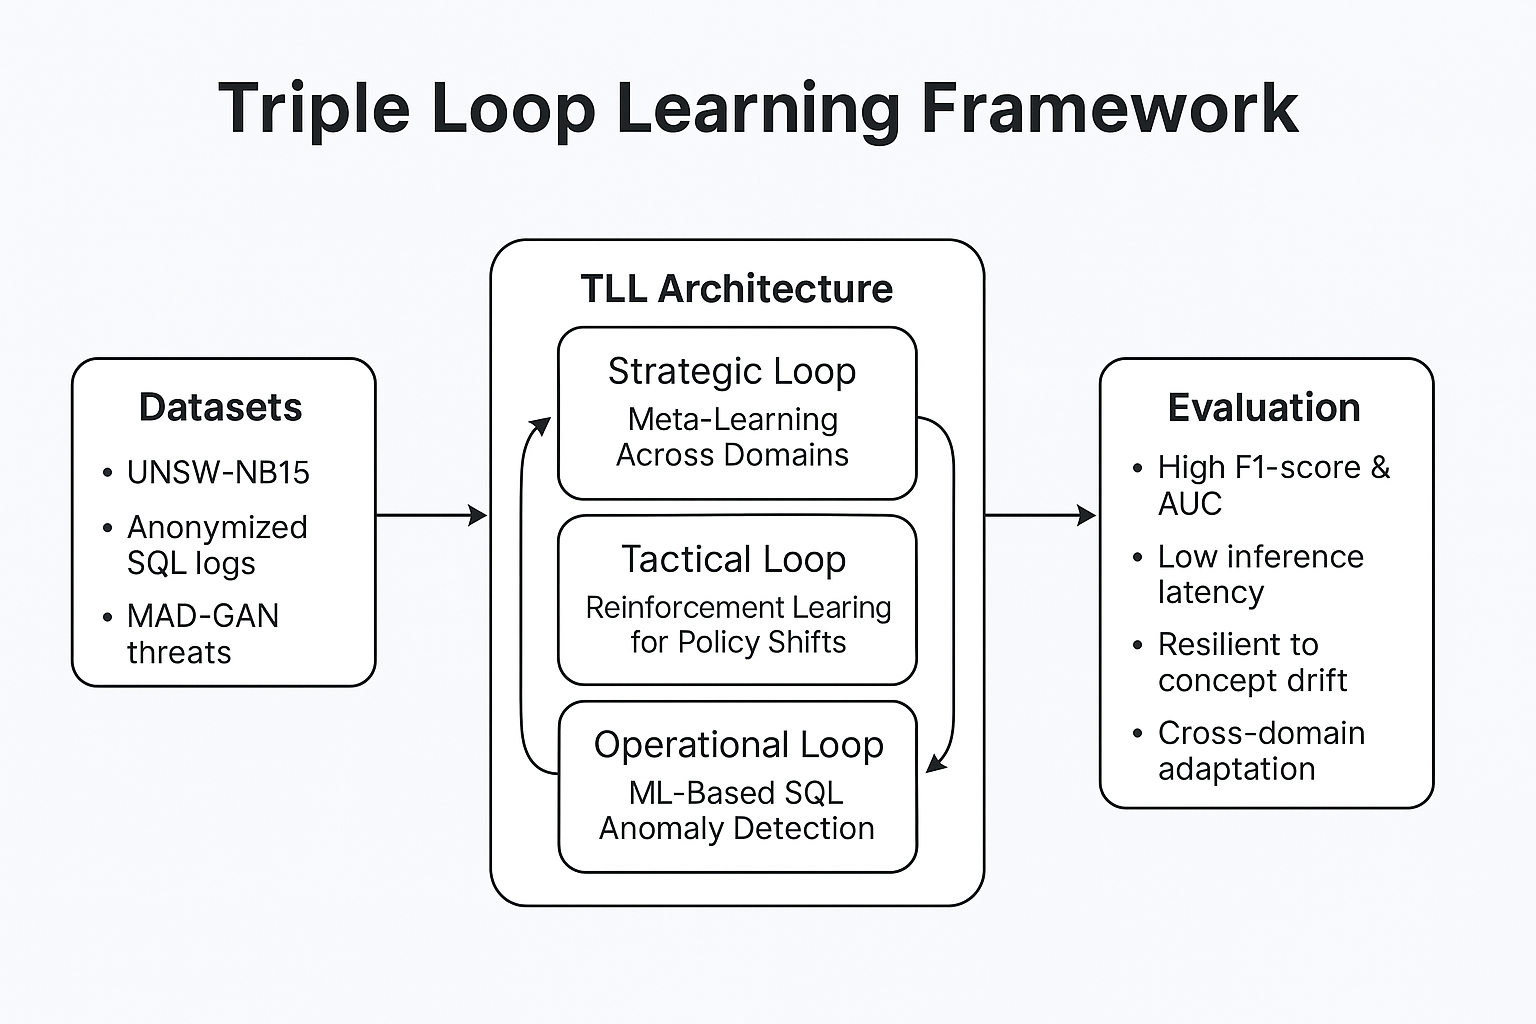
\includegraphics[width=\linewidth]{images/Triple_Loop_Learning_Framework_Diagram.png}
\end{block}
\end{column}

% Column 2
\begin{column}{0.32\textwidth}
\begin{block}{Materials}
\textbf{Datasets Used:}
\begin{itemize}
    \item UNSW-NB15: 2.54M labeled flow records
    \item Real SQL logs (1.2M entries)
    \item Adversarial MAD-GAN samples
\end{itemize}
\end{block}

\begin{block}{Results}
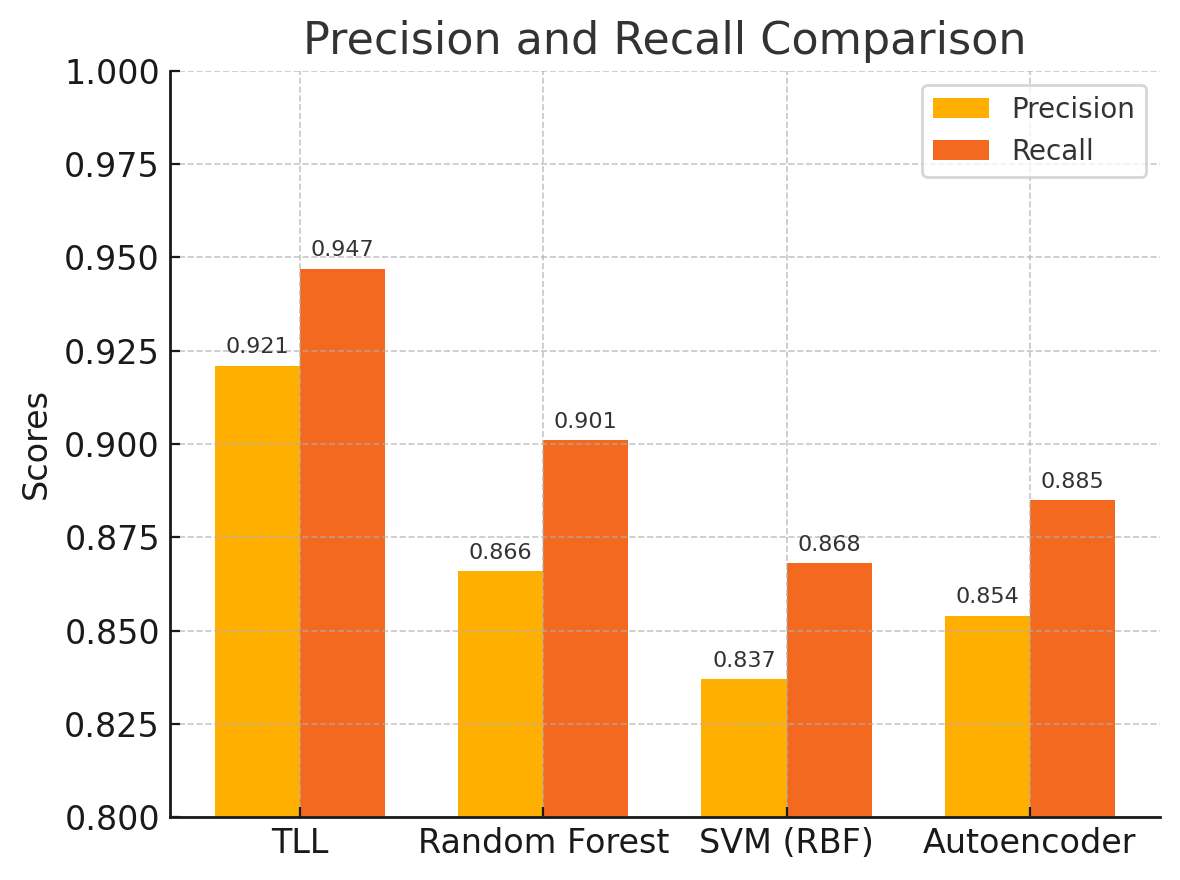
\includegraphics[width=\linewidth]{images/precision_recall_bar.png}
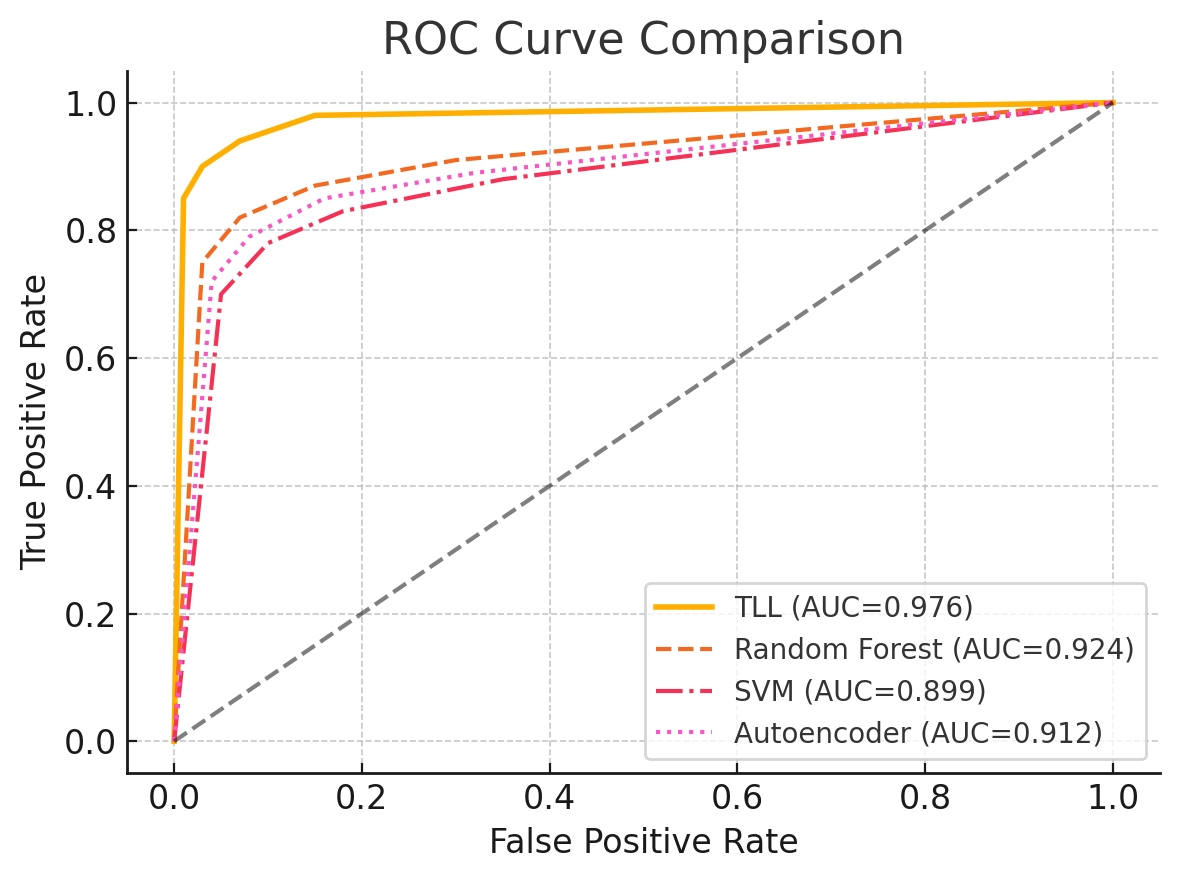
\includegraphics[width=\linewidth]{images/roc_curve_tll.png}
\textbf{Metrics:}
\begin{itemize}
    \item F1-score: \textbf{0.934}
    \item AUC: \textbf{0.976}
    \item Latency: \textbf{84ms/query}
\end{itemize}
\end{block}
\end{column}

% Column 3
\begin{column}{0.32\textwidth}
\begin{block}{Conclusion}
\begin{itemize}
    \item TLL outperforms baseline ML models in detection and latency.
    \item RL reduces false positives by 37\%.
    \item MAML enables generalization across institutions with limited training data.
\end{itemize}
\end{block}

\begin{block}{Deployment}
Dockerized and SIEM-compatible. Runs under 60\% GPU load for high-throughput environments.
\end{block}

\begin{block}{Contact \& Code}
\href{mailto:a09726537@unet.univie.ac.at}{a09726537@unet.univie.ac.at} \\ 
GitHub: \href{https://github.com/a09726537/tll-rdbms}{github.com/a09726537/tll-rdbms}
\end{block}
\end{column}

\end{columns}

\vspace{1cm}
\begin{block}{Acknowledgments}
Advised by Univ.-Prof. Dr. Dr. Gerald Quirchmayr, University of Vienna. Compliant with GDPR. All experimental logs anonymized.
\end{block}

\end{frame}

\end{document}
